\chapter{Zajednička AST apstrakcija za imperativne jezike}
\label{chp:MyAST}

Kao što je opisano u odeljku \ref{sec:Paradigms}, dosta različitih "pod-paradigmi" potiče iz imperativne paradigme. Strukturna, proceduralna i skript paradigma, iako naizgled različite, poseduju veliki broj sličnih osobina i koncepata. Svaki programski jezik ima svoju gramatiku i na osnovu toga ima svoja gramatička pravila koja se oslikavaju u apstraktnim sintaksnim stablima tih jezika. Na slikama \ref{fig:ASTLua} i \ref{fig:ASTGo} se mogu videti razlike u strukturi AST-a za jezike \texttt{Lua} i \texttt{Go}, kao primeri skript odnosno proceduralne paradigme.

\begin{figure}[h!]
    \centering
        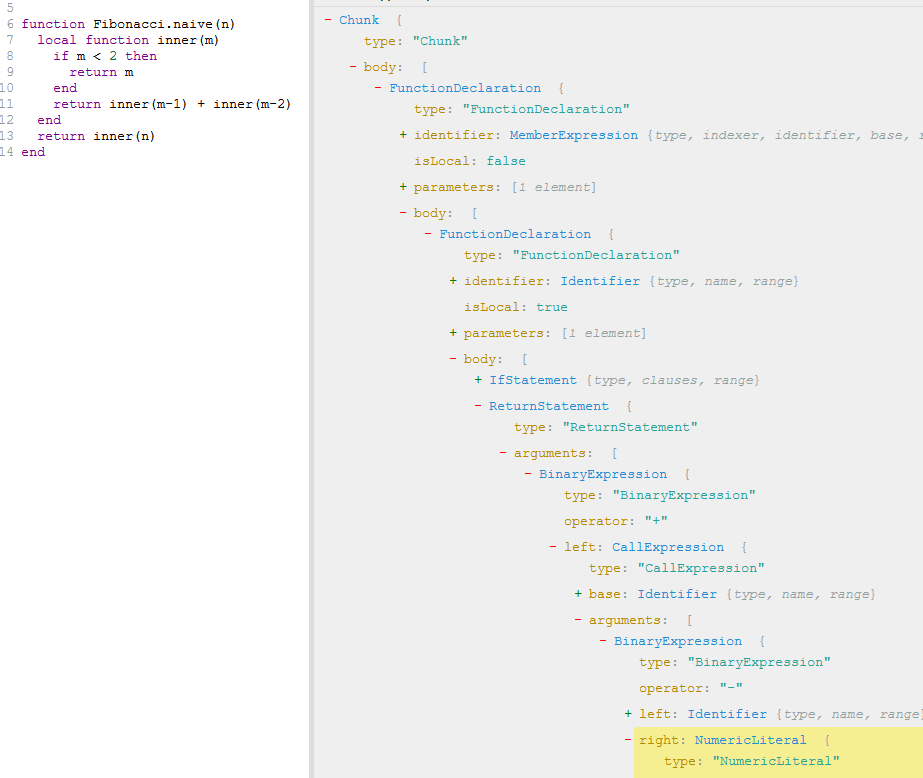
\includegraphics[scale=0.6]{images/ast_lua.png}
    \caption{Prikaz AST-a isečka koda pisanog u programskom jeziku Lua. Prikazano putem \url{https://astexplorer.net/}}
    \label{fig:ASTLua}
\end{figure}

\begin{figure}[h!]
    \centering
        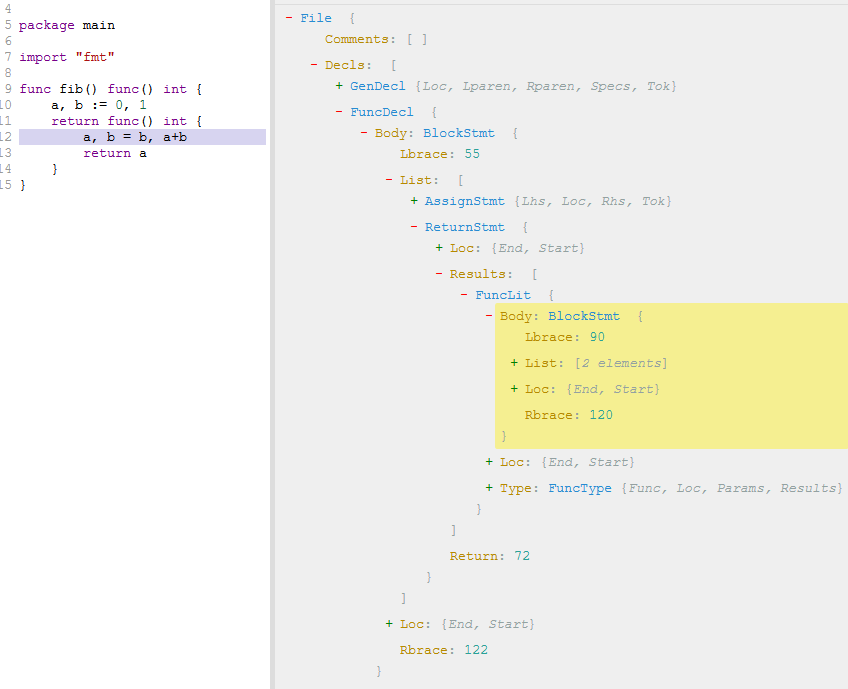
\includegraphics[scale=0.7]{images/ast_go.png}
    \caption{Prikaz AST-a isečka koda pisanog u programskom jeziku Go. Prikazano putem \url{https://astexplorer.net/}}
    \label{fig:ASTGo}
\end{figure}

U ovoj poglavlju će biti predstavljena AST apstrakcija dizajnirana tako da je uz pomoć nje moguće predstaviti kodove proizvoljnog imperativnog programskog jezika. To uključuje i skript jezike koji, kako će biti pokazano u ovom radu, mogu da se posmatraju na istom nivou kao i svoji proceduralni "rođaci".

Kako bi se kreirala smislena apstrakcija stabla parsiranja, potrebno je identifikovati bitne informacije u stablu parsiranja ali i koncepte same gramatike koji su od značaja. Najjednostavnije rešenje je mimikovati čvorove stabla parsiranja, ukoliko su gramatička pravila kreirana tako da oslikaju koncepte jezika koji gramatika definiše. Na primer, ukoliko u gramatici imamo pravilo \texttt{deklaracija} sa alternativama \texttt{deklaracijaPromenljive} i \texttt{deklaracijaFunkcije}, možemo kreirati apstraktni koncept \texttt{Deklaracija} sa konkretizacijama \texttt{DeklaracijaPromenljive} i \texttt{DeklaracijaFunkcije}. Kako se definišu deklaracije promenljivih i funkcija zavisi dalje od definicija pravila \texttt{deklaracijaPromenljive} i \texttt{deklaracijaFunkcije}. Naravno, nije uvek moguće primeniti ovakav postupak. Takođe, nekada u gramatici definišemo pomoćna pravila kako bismo se izborili sa rekurzijom ili izbegli neke tipove rekurzije - ta pravila ne bi trebalo da imaju odgovarajuće tipove u apstrakciji. 

Pošto su u pitanju gramatike programskih jezika, onda je jasno da dosta različitih gramatika dele slične koncepte i da je moguće definisati tipove čvorova koji odgovaraju tim konceptima. Neki od njih mogu biti: naredba, izraz, deklaracija, poziv funkcije, dodela... Jasno, postoji i hijerarhija između navedenih koncepata - poziv funkcije se može smatrati kao samostalna naredba ali može biti i deo izraza. Dakle, treba biti jako pažljiv u definisanju hijerarhije tako da ne dozvoli nešto što u opštem slučaju ne bi trebalo da bude dozvoljeno (npr. ako je dozvoljeno višestruko nasleđivanje i poziv funkcije je i naredba ali i izraz, onda se izrazi u kojima figurišu pozivi funkcija sastoje od više naredbi, što nema smisla.).

Osim naredbi i izraza (koje vezuju operatori), kao osnovnih koncepata imperativnih jezika, deklaracije se ne pojavljuju u skript jezicima. Moguće je, međutim, posmatrati i promenljive u kodovima skript jezika kao promenljive deklarisane pre trenutka njihove upotrebe - detaljnije opisano u \ref{sec:MyASTDeclarationNodes}. Što se tiče njihovog tipa, može biti dozvoljena promena istog, ili, kako je izabrano u ovom radu, biće iskorišćen specijalni tip od kog potiču svi ostali tipovi.

\begin{figure}[h!]
    \centering
        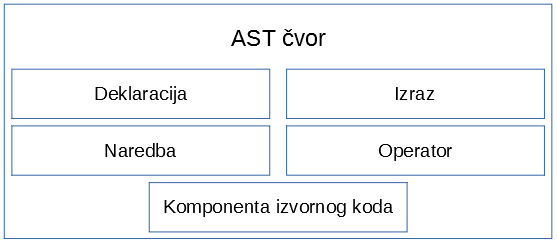
\includegraphics[scale=0.7]{images/nodes.png}
    \caption{Prikaz osnovnih vrsta AST čvorova.}
    \label{fig:ASTNode}
\end{figure}

Na slici \ref{fig:ASTNode} se mogu videti osnovni tipovi AST čvorova zasnovani na konceptima opisanim iznad. U nastavku će po odeljcim biti detaljnije opisan svaki od tipova AST čvorova sa slike.

\section{Čvorovi deklaracija}
\label{sec:MyASTDeclarationNodes}

Kao što je opisano u odeljku \ref{sec:Paradigms}, u striktno tipiziranim proceduralnim jezicima promenljive i funkcije koje se koriste se moraju deklarisati pre trenutka njihovog korišćenja. Prateći kvalifikatori (statičnost, konstantnost itd.) i modifikatori pristupa (javni, privatni itd.) će se u nastavku nazivati \emph{specifikatori deklaracije} (engl. \emph{declaration specifiers}). Nakon specifikatora deklaracije dolazi konkretan \emph{deklarator}, koji ima specifičan oblik u zavisnosti od toga šta se deklariše. Oba imena su uzeta po uzoru na imena pravila gramatike programskog jezika C. 

Veliki broj proceduralnih jezika dozvoljava deklarisanje više promenljivih odjednom koje dele iste specifikatore deklaracije. Stoga specifikatore neće pratiti jedan deklarator, nego \emph{lista deklaratora}. Takođe, deklaratori u listi ne moraju biti samo deklaratori promenljivih - moguće je deklarisati i nizovnu promenljivu zajedno sa deklaracijama običnih promenljivih. Na slici \ref{fig:DeclarationParts} se može videti dekompozicija deklaracije promenljive i niza u različitim proceduralnim programskim jezicima a na slici \ref{fig:DeclarationNodes} uočena hijerarhija sa podvrstama deklaratora.

\begin{figure}[h!]
\centering
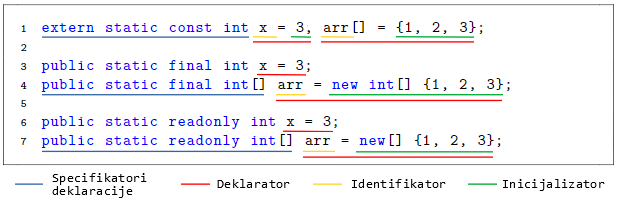
\includegraphics[scale=0.8]{images/declaration_decomposition.png}
\caption{Delovi deklaracije promenljive i niza prikazani na isečcima koda pisanog u programskim jezicima C, Java i C\#.}
\label{fig:DeclarationParts}
\end{figure}

\begin{figure}[h!]
\centering
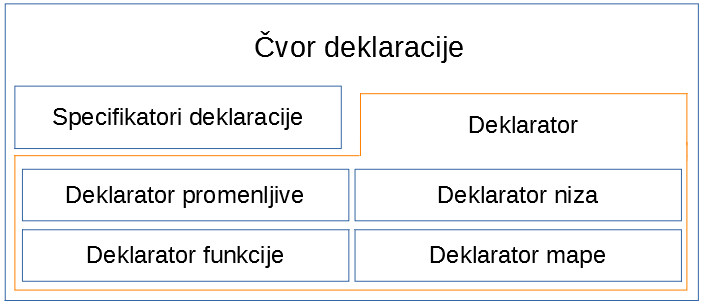
\includegraphics[scale=0.5]{images/declaration_nodes.png}
\caption{Prikaz vrsti AST čvorova deklaracije.}
\label{fig:DeclarationNodes}
\end{figure}

Kao što je prikazano na slici \ref{fig:DeclarationParts}, specifikatori deklaracije pokrivaju kvalifikatore, specifikatore pristupa i ime tipa. Pošto se pravi zajednička apstrakcija, potrebno je uočiti ekvivalenetne ključne reči u različitim programskim jezicima - u primeru sa slike to su \texttt{const}, \texttt{final} i \texttt{readonly}. Imena tipova u programskim jezicima Java i C\# uzeta su po uzoru na programski jezik C, tako da tu ne vidimo razlike. U opštem slučaju, moguće je definisati mapiranje imena tipa u apstraktni tip. Ukoliko, na primer, posmatramo tipove koji predstavljaju realne brojeve, osim tipova \texttt{float} i \texttt{double}, postoji i tip \texttt{decimal} prisutan u programskom jeziku C\# \footnote{Tip \texttt{decimal} predstavlja 128-bitni realan broj sa povećanom veličinom mantise a smanjenom veličinom eksponenta u odnosu na tip \texttt{double}. Koristi se u numeričkm izračunavanjima gde preciznost primitivnih tipova realnih brojeva nije dovoljna.}. Sva tri ova tipa mogu da se posmatraju na istom nivou apstrakcije kao tip realnih brojeva. Za korisnički definisane tipove isto ne može da se primeni.

Deklaratori za proceduralne jezike mogu biti deklaratori promenljive, niza ili funkcije i od toga zavisi njihov sastav. Svi deklaratori moraju sadržati informaciju o idenfitikatoru. Ukoliko je reč o deklaratoru niza, dodatno se očekuje i oznaka za niz (obično par srednjih zagrada - \texttt{[]}) i opcioni izraz koji predstavlja dimenziju niza, obično unutar oznake niza. Ukoliko je reč o deklaratoru funkcije, pored identifikatora se očekuje i lista parametara funkcije obično navedena unutar para običnih zagrada. Lista parametara funkcije se može posmatrati rekurzivno - svaki parametar se može posmatrati kao varijanta deklaracije - sadrži specifikatore deklaracije (koji uključuju i tip) i deklarator, s tim što u ovom slučaju nije dozvoljeno da taj deklarator bude deklarator funkcije (pošto funkcije nisu građani prvog reda u imperativnoj paradigmi). 

Deklaratori promenljive i niza mogu dodatno sadržati i \emph{inicijalizator}. Inicijalizator možemo posmatrati kao opcioni izraz u slučaju deklaratora promenljive. U slučaju deklaratora niza, inicijalizator može biti lista izraza. Deklaratori funkcije ne mogu imati inicijalizatore.

U skript jezicima su uobičajeno podržane strukture podataka kao što su skupovi i mape. Stoga, kako bi se i mape mogle predstaviti apstraktno, dodat je tip deklaratora koji predstavlja deklarator mape. Mapa se sastoji od skupa ključeva pri čemu je svakom ključu dodeljena vrednost ne nužno istog tipa kao što je tip ključa. Mape postoje i u proceduralnim jezicima, ali ključna razlika je ta što tipovi u skript jezicima nisu striktni - ključevi međusobno, ali i vrednosti mogu biti različitog tipa. Vredi naglasiti da se mape mogu porediti sa objektima određenih klasa - svaki objekat se može serijalizovati u mapu gde su ključevi imena javnih atributa klase a vrednosti su vrednosti javnih atributa objekta koji se serijalizuje. Neki jezici (kao što je Python), imaju funkcije koje od objekta vraćaju baš ovakvu mapu. Ova ideja se dalje može proširiti kako bi se serijalizovale i metode klase, označila statička i privatna polja kao i sačuvale informacije o definisanim konstruktorima. Zatim je moguće porediti mape definisane u skript jezicima sa objektima iz proceduralnih jezika.

Na slici \ref{fig:MyASTExampleCDeclaration} se mogu videti kreirani AST za nekoliko deklaracija pisanih u programskom jeziku C a na slici \ref{fig:MyASTExampleLuaDeclaration} se može isto videti demonstracija \emph{automatske deklaracije} promenljivih za skript programski jezik Lua. Naime, pre prvog pojavljivanja identifikatora veštački će biti deklarisan taj identifikator, kako bi razlika između AST-ova dobijenih iz proceduralnih i skript jezika bila što manja. U ovom slučaju će se deklaracija i dodela spojiti u deklaraciju sa inicijalizatorom.

\begin{figure}[h!]
\begin{lstlisting}
extern int y = 3;
static int arr[5] = { 1 };
\end{lstlisting}
\centering
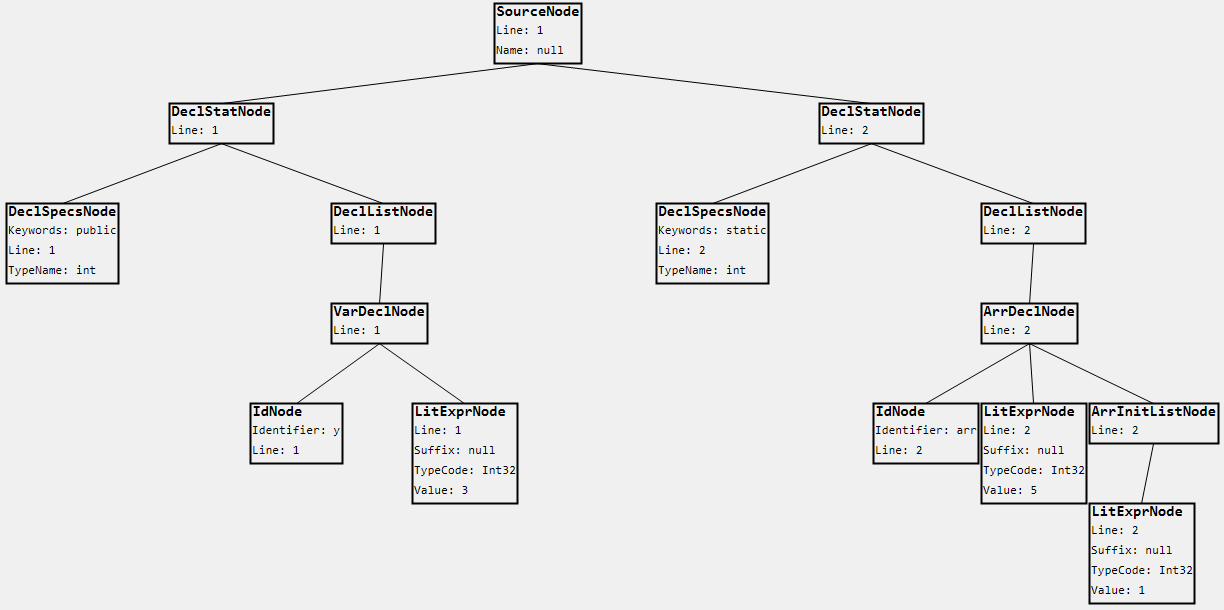
\includegraphics[scale=0.48]{images/c_ast_decl2.png}
\caption{Primer deklaracije promenljive i niza u programskom jeziku C i odgovarajući AST.}
\label{fig:MyASTExampleCDeclaration}
\end{figure}

\begin{figure}[h!]
\begin{lstlisting}
arr = { 1, 2 }
dict = { a = 1 }
\end{lstlisting}
\centering
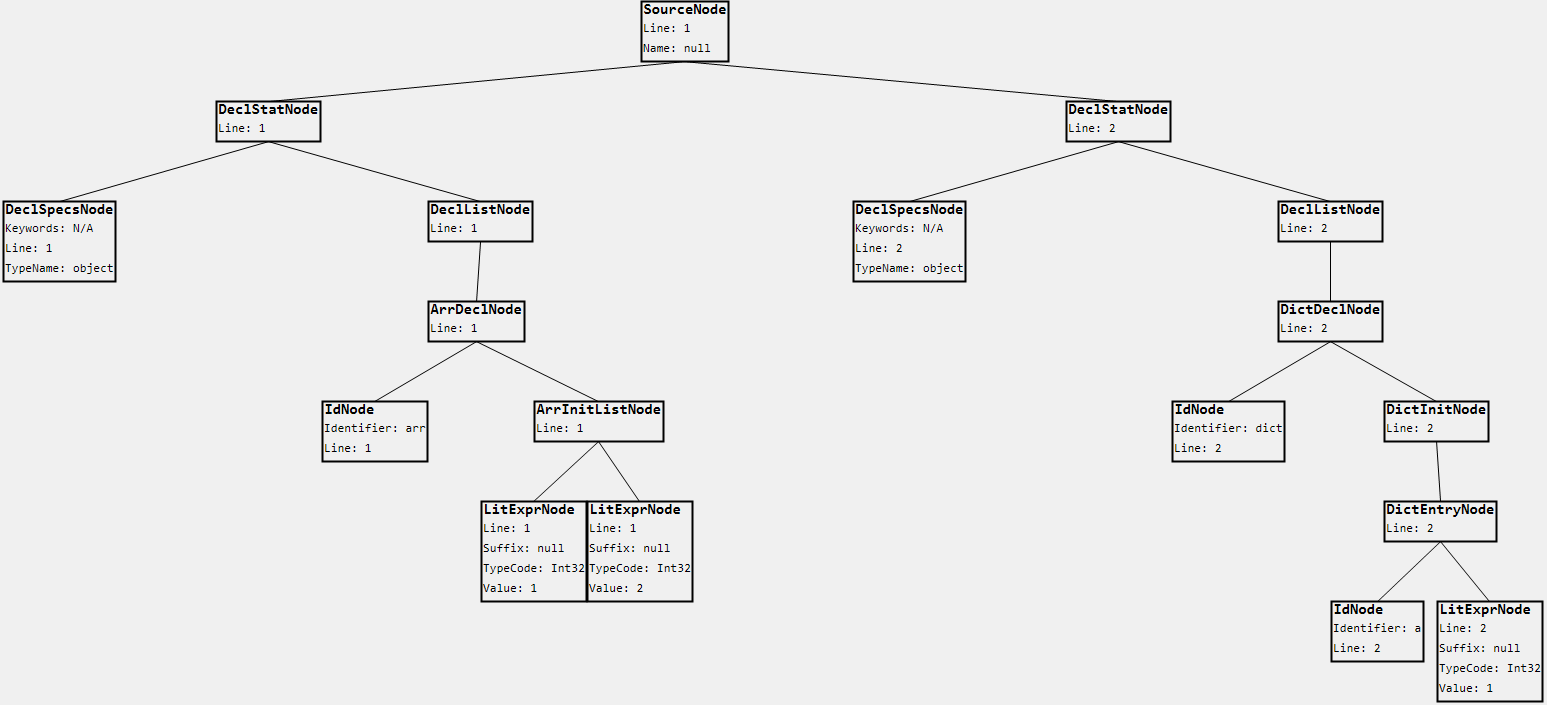
\includegraphics[scale=0.4]{images/lua_ast_decl.png}
\caption{Primer deklaracije promenljive i niza u programskom jeziku Lua i odgovarajući AST.}
\label{fig:MyASTExampleLuaDeclaration}
\end{figure}


\section{Čvorovi operatora}
\label{sec:MyASTOperatorNodes}

Svrha operatora je da vezuju izraze i da tako grade nove izraze. Operator se karakteriše simbolom i \emph{arnošću}, tj. brojem argumenata koje taj operator prima. Na osnovu arnosti, svaki operator se može apstraktno posmatrati kao članica grupe operatora sa istom arnošću. Na slici \ref{fig:OperatorNodes} se može videti hijerarhija operatora korišćena dalje u apstrakciji. Binarni operatori zahtevaju dva operanda i pišu se infiksno, dok unarni zahtevaju jedan operand i pišu se prefiksno. Ternarni operatori koji postoje u nekim programskim jezicima nisu razmatrani jer se mogu posmatrati kao druge strukture \footnote{Na primer, ternarni operator \texttt{?:} prisutan u jezicima zasnovanim na sintaksi programskog jezika C se može zameniti naredbom uslovnog grananja.}. 

\begin{figure}[h!]
\centering
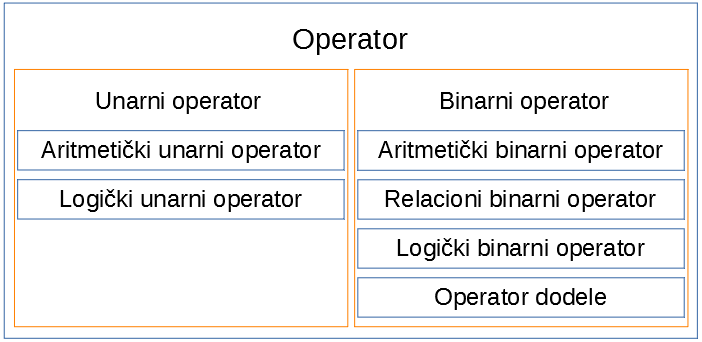
\includegraphics[scale=0.5]{images/operator_nodes.png}
\caption{Podela operatora na osnovu njihove arnosti.}
\label{fig:OperatorNodes}
\end{figure}

Unarni aritmetički operatori su unarni operatori koji figurišu u aritmetičkim izrazima, npr. operator promene znaka, operator bitovske negacije \emph{Bitovski izrazi se mogu posmatrati kao vrsta aritmetičkih izraza}, operatori kastovanja ili inkrementiranja odnosno dekrementiranja. Unarni logički operatori su unarni operatori koji figurišu u logičkim izrazima, npr. operator negacije. Možemo sve ove unarne operatore posmatrati apstraktno ukoliko definišemo unarni operator kao strukturu koja definiše unarnu funckiju koja transformiše svoj argument na osnovu logike konkretnog unarnog operatora. Tip argumenta i povratne vrednosti pomenute funkcije zavisi od tipa unarnog operatora - aritmetički unarni operatori mogu primiti vrednost bilo kog tipa \footnote{Ne postoji ograničenje na brojevne tipove jer se u nekim jezicima operatori mogu predefinisati tako da rade i za korisnički definisane tipove (engl. \emph{operator overloading}).} i vračaju vrednost proizvoljnog, ne nužno istog tipa; dok unarni logički operatori primaju i vraćaju bulovsku vrednost \footnote{U nekim programskim jezicima postoji implicitna konverzija brojevnih tipova u bulovski tip, što se jednostavno može posmatrati kao poređenje vrednosti po jednakosti sa nulom.}. Koristeći ovaj pristup, nije potrebno praviti novi AST čvor za svaki mogući operator, već je dovoljno da postoji samo jedan čvor koji predstavlja unarni operator. Ovakav pristup odgovara varijanti AST sa regularnošću (videti sliku \ref{fig:ASTVariants}), omogućava opisivanje proizvoljnih operatora i nije vezan za konkretnu programsku paradigmu.

Binarni aritmetički operatori su binarni operatori koji figurišu u aritmetičkim izrazima, npr. operatori koji odgovaraju matematičkim operacijama ali i bitovski binarni operatori. Binarni relacioni operatori su binarni operatori koji figurišu u relacionim izrazima, npr. operatori poretka ($<$, $>$, $\leq$, $\geq$) i poređenja po jednakosti ili različitosti ($=$, $\neq$). Binarni logički operatori su binarni operatori koji figurišu u logičkim izrazima, npr. bulovske operacije ($\wedge$, $\vee$). Slično kao i za unarne operatore, moguće je apstraktno posmatrati sve binarne operatore tako što ih definišemo kao strukturu koja definiše binarnu funkciju koja transformiše argumente na osnovu logike konkretnog binarnog operatora. Tip argumenata i povratne vrednosti te funkcije zavisi od tipa binarnog operatora, kao i u slučaju unarnih operatora - aritmetički binarni operatori primaju dva argumenta proizvoljnog tipa i vraćaju rezultat proizvoljnog, ne nužno istog tipa; relacioni binarni operatori primaju iste tipove argumenata kao i aritmetički binarni operatori, međutim povratna vrednost mora biti bulovskog tipa; dok logički binarni operatori zahtevaju da argumenti i povratna vrednost budu bulovskog tipa. Pritom, na prvi pogled nije jasno kako se operator dodele može uklopiti u ovaj šablon ali, na osnovu toga da je dodela zapravo sporedni efekat i da se posmatra kao izraz čija je vrednost jednaka vrednosti izraza sa desne strane operatora, može se primeniti isti princip kao i za aritmetičke binarne izraze. Neki programski jezici dozvoljavaju i složene operatore dodele, koji se mogu dekomponovati na više jednostavnijih izraza.

\section{Čvorovi izraza}
\label{sec:MyASTExpressionNodes}

\pangrami

\section{Čvorovi naredbi}
\label{sec:MyASTStatementNodes}

Naredbe su najkomplikovanije za apstrahovanje zbog njihove raznovrsnosti. Programski jezici često uvode nove sintaksne strukture i naredbe koje nisu do tada viđene u ostalim jezicima. Uprkos svemu tome, ipak je moguće uočiti neke sličnosti sa već postojećim konceptima i svesti ih na isti nivo. Na slici \ref{fig:StatementNodes} se mogu videti tipovi apstraktnih konstrukcija koje će se koristiti da bi se predstavile naredbe.

\begin{figure}[h!]
\centering
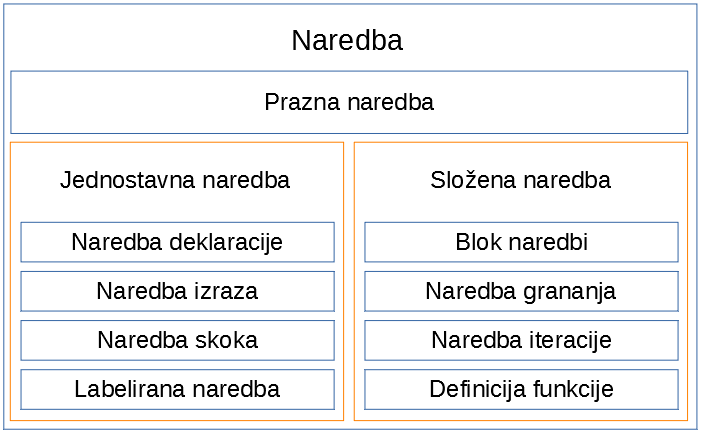
\includegraphics[scale=0.5]{images/statement_nodes.png}
\caption{Vrste čvorova naredbi.}
\label{fig:StatementNodes}
\end{figure}

Veliki broj programskih jezika podržava praznu naredbu, sa semantikom ne izvršavanja nikakvih operacija. U programskim jezicima koji su zasnovani na sintaksi jezika C, praznu naredbu navodimo samo korišćenjem simbola za kraj naredbe (\texttt{;}), dok u programskom jeziku Python koristimo ključnu reč \texttt{pass}. 

Naredbe su podeljene na \emph{jednostavne} i \emph{složene}, koje se sastoje od više drugih naredbi. Primer jednostavne naredbe može biti deklaracija promenljive, dok primer složene naredbe može biti definicija funkcije koja se sastoji od više jednostavnih deklaracija ali možda i drugih složenih naredbi kao što su grananja i petlje.

Jednostavne naredbe uključuju naredbe deklaracije i izraza. Razlog zašto se deklaracije i izrazi opet pojavljuju je taj što izrazi sami po sebi mogu biti deo drugih naredbi. Ukoliko se naredba sastoji samo od izraza, onda nju zovemo naredbom izraza. Primer može biti izraz dodele --- vrednost izraza dodele se može koristiti u drugim izrazima ali, ukoliko samo želimo da izvršimo dodelu i ništa više u okviru iste naredbe, onda izraz dodele "umotavamo" u naredbu izraza. Slično važi i za deklaracije, ukoliko razmotrimo idiomsku \texttt{for} petlju (od standarda C99) --- moguće je deklarisati promenljive koje se koriste unutar ciklusa ali to nije naredba deklaracije već deklaracija koja se koristi unutar druge naredbe. 

Naredbe se mogu označiti, po uzoru na koncept \emph{labele} u imperativnim jezicima --- identifikatora koji označava lokaciju u izvornom kodu. Labele se u imperativnim jezicima najviše koriste da bi se izvršili skokovi na određene lokacije u kodu ali su takođe prisutne i u proceduralnim jezicima (npr. kroz naredbu višestrukog grananja --- \texttt{switch} ili u nekim jezicima \texttt{case}). Labelirana naredba se sastoji od naredbe i identifikatora koji predstavlja labelu. 

Naredbe skoka se koriste obično u paru sa labeliranim naredbama, ali to ne mora uvek biti slučaj. Iako ove čvorove koristimo da bismo predstavili naredbe skoka prisutne u imperativnim jezicima, one predstavljaju i naredbe prekida (\texttt{break} ili \texttt{continue}) ili povratka vrednosti funkcije (\texttt{return}). U slučaju da je u pitanju skok na određenu labelu, onda se sastoji i od identifikatora koji predstavlja labelu na koju se skače. Ukoliko je u pitanju naredba prekida, nisu potrebne nikakve dodatne informacije (mada se i u tom slučaju može iskoristiti činjenica da su u pitanju skokovi pa se može labelirati petlja na koju se odnosi naredba prekida). U slučaju povratka vrednosti funcije, sadrži opcioni izraz čija vrednost predstavlja povratnu vrednost funkcije.

Složene naredbe se sastoje od više drugih naredbi (ne nužno samo od jednostavnih). Često je potrebno izvršiti više naredbi u okviru jednog konteksta i za to se koristi blok naredba. Blok naredba grupiše više drugih naredbi u jednu. Blok naredba se u proceduralnim jezicima obično navodi eksplicitno, za programski jezik C pomoću velikih zagrada (\texttt{\{\}}), a za skript jezike često je implicitna ili se navodi korišćenjem različitih nivoa indentacije (Python).

Naredbe uslovnog grananja se sastoje od \emph{uslova}, koji može biti relacioni ili logički izraz, naredbe koja se vrši ukoliko je uslov ispunjen (\emph{then} grama), i opciono naredbe koja se izvršava ako uslov nije ispunjen (\emph{else} grana). Rezultat uslovnog izraza, iako mora biti istinitosna vrednost, je dozvoljeno da bude bilo kog tipa (dakle nema ograničenja samo na relacione i logičke izraze) iz razloga što određeni programski jezici dozvoljavaju automatsku konverziju brojevnih tipova u logički (C). Štaviše, nekada je moguća i implicitna konverzija određenih tipova u logički tip definisanjem implicitnih operatora konverzije (C\#). Zato će u apstrakciji uslov biti bilo koji izraz. Što se \emph{then} i \emph{else} grana tiče, one mogu biti bilo koje naredbe, ali zarad konzistentnosti će obe biti blokovi naredbi. Na slici \ref{fig:MyASTExampleStatement} se može videti AST za naredbu grananja.

\begin{figure}[h!]
\begin{lstlisting}
do                               something()
    something()                  while (condition) do
while (condition)                    something()
\end{lstlisting}
\begin{lstlisting}
repeat                           something()
    something()                  while (not condition) do
until (condition)                    something()
\end{lstlisting}
\caption{Procedura svođenja ređih tipova petlji (levo) na \emph{while} petlju (desno) prikazana u pseudo-jeziku.}
\label{fig:ASTIterationStatements}
\end{figure}

Naredbe iteracije imaju raznovrsni oblik u programskim jezicima. Najčešće podržane naredbe iteracije su \emph{for}, \emph{while} i \emph{foreach} petlje. U opštem slučaju, dovoljno je koristiti samo jedan tip petlji, ali zarad jednostavnosti i prisutnosti ovih tipova u velikoj većini programskih jezika oba će biti podržana. Ostali tipovi petlji, kao što su \emph{do-while} ili \emph{repeat-until} petlje, će se svoditi na njih. \emph{do-while} petlja se može svesti na \emph{while} petlju jednostavnim ponavljanjem tela petlje pre same petlje i kreiranjem obične \emph{while} petlje sa istim uslovom i telom. Slično se može uraditi i za \emph{repeat-until} petlju, s tim što je potrebno samo negirati uslov u dobijenoj \emph{while} petlji. Ovaj proces je ilustrovan na slici \ref{fig:ASTIterationStatements}.

\begin{figure}[h!]
\centering
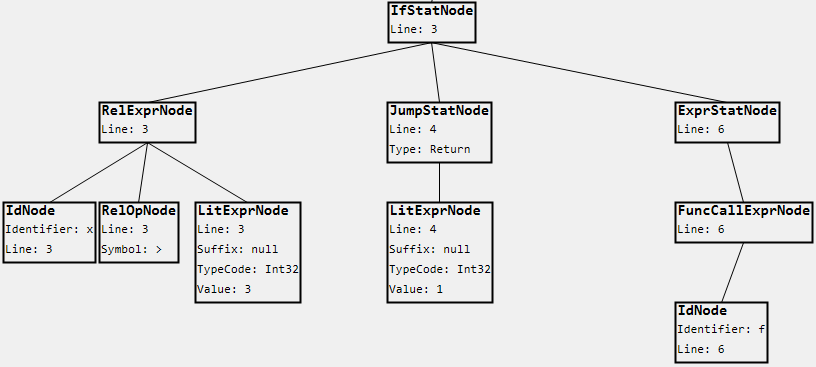
\includegraphics[scale=0.7]{images/ast_stat.png}
\caption{AST naredbe grananja.}
\label{fig:MyASTExampleStatement}
\end{figure}

